\documentclass[11pt, a4paper]{article}
% \documentclass[11pt, a4paper]{scrartcl}

\usepackage[a4paper,lmargin={3cm},rmargin={3.5cm}, tmargin={2.5cm},bmargin = {2.5cm}]{geometry}
\usepackage{setspace}
\usepackage{indentfirst}
    %\onehalfspacing
    \usepackage{enumitem}
    \usepackage{amsmath, amssymb}
\usepackage{graphicx}

\newcommand{\mh}[1]{\noindent\emph{#1}}
\newcommand{\Ssa}{S_{\sigma\alpha}}
\newcommand{\Stsa}{S^t_{\sigma\alpha}}
\newcommand{\sa}{{\sigma\alpha}}
\newcommand{\given}[1][]{\:#1\vert\:}
\newcommand{\Sm}{\Stsa~m^t_{\sa}}
\newcommand{\CI}{\mathrel{\perp\mspace{-10mu}\perp}}
\newcommand{\nCI}{\centernot{\CI}}
\newcommand{\Var}{\mathrm{Var}}
\renewcommand{\i}[1]{\emph{#1}}
\renewcommand{\a}{\alpha}

\usepackage[backend=biber, authordate, ibidtracker=context]{biblatex-chicago}
\addbibresource{preemption.bib}

\title{\textbf{How to Deal With Expert Testimony?} \\Preemption View and Total Evidence View tested in the Olsson and Vallinder Model for Social Networks }
\author{Class Paper: Formal Methods II \\ MCMP @ LMU Munich \\ Conrad Friedrich \\ \texttt{conradfriedrich@posteo.net}}

\begin{document}

\maketitle
\abstract{Is expert testimony just another source of evidence? Or does it have an epistemically special status that should be reflected in how we rationally update our credences? In this paper, I compare two different strategies of dealing with expert testimony, the standard Bayesian way and another, called the Preemption View of authority testimony. To this end I extend the Olsson Vallinder model for social networks to accommodate this recently proposed strategy. Given some plausible assumptions, I surprisingly find that the result do not favor the Preemption View, although of course caveats apply and are addressed. }

\section{Introduction}
How to deal with expert testimony? Mention Goldman, Elga etc.

Show position by Kelly
Show position of Constantin and Grundmann

Show need to make this precise. In the case of preemption view, how to model? 
kelly's TEV for credences is just the same as Bayesianism 

How to evaluate the rational strategy formally?
Epistemic Value!

\section{Model Description}

The Model used in this paper follows the one proposed by \textcite{Olsson2013} rather closely. I adopt most of their formalizations and assumptions. To enable the reader to make use of the derivations in \textcite{Angere2010}, I adopt their notations as well. I summarize the model, describe how I use it for the present purposes and make note of any deviation.

The core entities of the model are \i{agents} and their properties. Agents can be connected to one another, such that they form a network. Since these connections enable communication and the agents are meant to represent people, this structure can be seen as a social network, represented in some form of graph representation through an adjacency matrix.

The model has certain starting parameters, which I describe below, and discrete time steps. Each of these enable the update of properties by the rules specified further below.

\subsection{Starting Parameters}

To keep things manageable, there is a single \i{true} target proposition $p$ which the agents have a credence $C^t_\alpha(p)$ towards. Each time step, agents can receive information from a \i{source}. These can be (i) other agents in the social network or (ii) their own inquiry. The objective chance that an agents inquires and gets it right is called that agent $\alpha$'s \i{aptitude}: $P(S_{\iota \alpha}p \given S_{\iota \alpha} \land p)$, where $S_{\iota \alpha}$ is the chance that agent $\alpha$ inquires for evidence, regardless of the results, and $S_{\iota \alpha} p$ the chance that she inquires and her inquiry yields $p$ as a result. The chance that she inquires at all, $P(S_{\iota \alpha})$, is called her \i{activity}. For the sake of simplicity, these chances are modeled as time invariant.

Sources can be more or less reliable. The reliability is assumed to be symmetric.
\[ 
R_{\sigma \alpha} =_{df.} P(\Ssa p \given \Ssa \land p) = P(\Ssa \neg p \given \Ssa \land \neg p)
\]
This is, of course, just the agent's aptitude. Note that the reliability of an agent is modeled continuously, in contrast to the binary full reliability/randomiser approach employed in \textcite[Chp. 3]{Bovens2003}, such that with a reliability value of less than $.5$ an agents inquiry would actually be negatively correlated with the truth.

Each agent trusts each source to a certain extent. This is expressed in the agent's credence in the reliability of the source:
\[ 
    C^t_{\alpha}(a \leqslant R_{\sa} \leqslant b) = \int_a^b \tau^t_{\sa}(\rho) d\rho
\]
where $\tau^t_{\sa}: [0,1] \rightarrow \mathbb{R}^+$ is a probability density function such that 
\[
    C^t_{\alpha}(0 \leqslant R_{\sa} \leqslant 1) =  \int_0^1 \tau^t_{\sa} (\rho) d(\rho) = 1
\]which is a very plausible requirement on a rational credence function.\footnote{Add Stuff here about the Olsson and Vallinder Model and how theirs is slightly different.}

\begin{description}
    \item[Example.] An agent $\alpha$ with a healthy trust in her own inquisitive abilities and who is not easily swayed in this trust may have a trust function $\tau^t_{\iota\alpha}$ described by a beta distribution
\[
    \tau^t_{\iota\alpha} (\rho) = \frac{1}{B(a,b)} \rho^{a - 1} {(1 - \rho)}^{b-1}
\]
with normalising beta function $B(a,b)$ and parameters $a, b$ chosen such that $\tau^t_{\iota\alpha}$ is densest around whatever a `healthy trust' amounts to, let's say 0.85 (cf.~Fig.~\ref{fig:trf}). Interestingly, the shape of the curve correlates with how resilient the function behaves upon updating. More on that below.
\end{description}

\begin{figure}[ht]
	\centering
    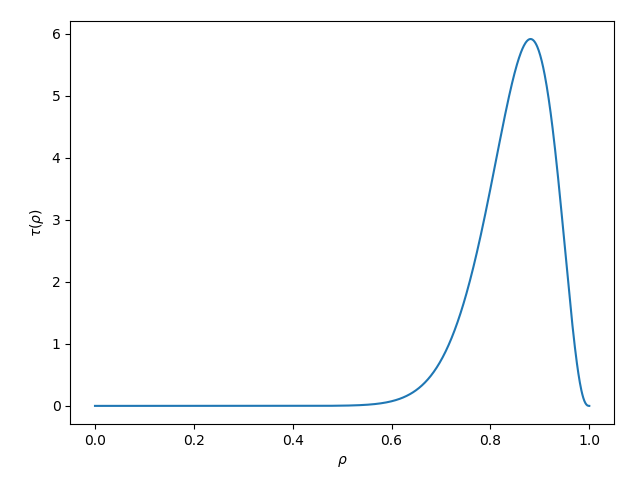
\includegraphics[width=0.5\textwidth]{Figure_1.png}
	\caption{Example beta distributed trust function with parameters a=LOOK b=UP\label{fig:trf}}
\end{figure}

Apart from inquiries, a source can also be another agent, through testimony. An agent $\alpha$ therefore trusts herself at time $t$ with $\tau^t_{\iota\alpha}$ and another agent $\beta$ with $\tau^t_{\beta\alpha}$.

The exchange of information and the evolution of the trust functions and the credences in $p$ are the most important going-ons in this model, which I'll summarize next.

\subsection{Inquiry and Communication} 

Time progress is modeled in discrete steps. At each time step, each agent updates her credence and her trust function. The new information which motivates these changes are messages from the sources, which the agent receives if
\begin{enumerate}[label = (\roman*)]
    \item the agent inquires herself with probability $P(S_{\iota\alpha})$. The result of the inquiry is determined by the agent's aptitude. Or,
    \item another agent $\beta$ is connected to agent $\alpha$ through the social network and decides to share her opinion. This is modeled, in slight deviation from the Olsson-Vallinder model, by the following conditions: 
        \begin{enumerate}[label = (\alph*)]
            \item Agent $\beta$ is sufficiently confident in $p$ resp. $\neg p$, determined by some fairly high threshold value for her credence, and
            \item agent $\beta$ received herself new information in the same time step. In the current implementation, this is only fulfilled by own inquiry.  
        \end{enumerate}
\end{enumerate}

EXPLAIN why only when new information!!

Testimony is, of course, a matter of language, and is most plausibly modeled as a binary judgment, that is, either $p$ or $\neg p$. While there are certainly interesting cases where the testimony involves credences or levels of confidences, e.g. \ a weather forecaster stating her belief in the chance of rain tomorrow, this does in my view not apply to  

\subsection{General Updating}

Each time step, the agents update their credences and trust functions. Updating the credences is based on new messages the agent received this time step: $\Stsa m^t_{\sa}$, where $m^t_{\sa}$ is the message that $\alpha$ received from $\sigma$ (which can represent $\alpha$'s own inquiry or another agent's testimony) at $t$, and is either $p$ or $\neg p$. An agents can receive multiple messages per time step, but only one message per source, so we have to account for that as well. 

In the central and most important deviation from the Olsson Vallinder model, I distinguish between the \i{Preemption} strategy and the \i{Total Evidence} strategy of dealing with expert testimony. In normal circumstances, both strategies involve the same standard bayesian updating rules, which I give in detail below. In the face of expert testimony they may differ, however, and I describe the requirements for differences as well as the differences themselves subsequently. 

The updating rule is given by conditionalisation:
\[
    C^{t+1}_\alpha (p) = C^t_\alpha (p \given \bigwedge_{\sigma \in \Sigma^t_\alpha} \Stsa m^t_{\sa}),
\]

where $\Sigma^t_\alpha$ is the set of sources that send a message to $\alpha$ at $t$.

With the assumption that sources are independent given the target proposition, the update calculates to
\begin{equation}
    \label{eq:upd}
    C^t_\a (p \given \bigwedge \Sm) = \\
     \frac{C^t_\a (p) \prod C^t_\a (\Sm \given p) }
    {C^t_\a (p) \prod C^t_\a (\Sm \given p) +  C^t_\a (\neg p) \prod C^t_\a (\Sm \given \neg p) }.
\end{equation}

Here, again, the product and big conjunct range over all sources with a message for the agent, the subscript omitted for legibility.   

The expressions about the reliability are given by:

\begin{align*}
    C^t_\a (\Stsa p \given p) &= C^t_\a (\Stsa) \langle \tau^t_{\sa} \rangle \\
    C^t_\a (\Stsa \neg p \given p) &= C^t_\a (\Stsa) \langle \bar{\tau}^t_{\sa} \rangle \\
    C^t_\a (\Stsa p \given \neg p) &= C^t_\a (\Stsa) \langle \bar{\tau}^t_{\sa} \rangle \\
    C^t_\a (\Stsa \neg p \given \neg p) &= C^t_\a (\Stsa) \langle \tau^t_{\sa} \rangle,
\end{align*}

where $\langle \tau^t_{\sa} \rangle $ is the expected value of trust function $ \tau^t_{\sa} $ and ${\langle \bar{\tau}^t_{\sa} \rangle =_{df.} 1 - \langle \tau^t_{\sa} \rangle}$.\footnote{Detailed and very helpful derivations of these equations can be found in \textcite{Angere2010}, although in places I could not agree with the results. I implemented the updating mechanism as presented in this paper. There is not much room to detail the finer points here, only this much: Angere's final result on page 22 for the credence update intuitively can't be right, since the expression as stated there does not depend on the actual content of the message, that is, $p$ or $\neg p$, anymore, and instead just updates regardless, rendering the network communication ineffective.} 

Upon receiving a message, the agent updates her trust function for that source depending on how well the message coheres with her own credence. The updated trust function can be calculated to
\[
    \tau^{t+1}_\sa = \tau^t_\sa (\rho) \frac{\rho \: C^t_\a (p) + (1 - \rho) C^t_\a (\neg p)}
    {\langle \tau^t_\sa \rangle C^t_\a(p) + \langle \bar{\tau}^t_\sa \rangle C^t_\a(\neg p)}
\]
if $m^t_{\sa} = p$, and 
\[
    \tau^{t+1}_\sa = \tau^t_\sa (\rho) \frac{\rho \: C^t_\a (\neg p) + (1 - \rho) C^t_\a (p)}
    {\langle \tau^t_\sa \rangle C^t_\a(\neg p) + \langle \bar{\tau}^t_\sa \rangle C^t_\a(p)}
\]
if $m^t_{\sa} = \neg p$. This entails that the trust an agents brings towards a source only changes with regard to the agents credence in p and the source's message whether p. This is one of the major shortcomings of the model, in my view, especially for the current purposes, as at no stage something like higher order evidence about the reliability of the source comes into play. 

Insert example with trust function development?

\subsection{Updating With Preemption}

In certain cases, an agent who pursues the preemptive strategy differs in her updating rule from what is described above, namely when she recognizes another agent as an epistemic authority. I modeled Constantin and Grundmann's requirements for the recognition of an epistemic authority in the following way. 
\begin{description} 
    \item[Epistemic Authority] An agent $\alpha$ recognizes another agent $\beta$ as an epistemic authority regarding proposition $p$ at time $t$ if and only if  
    \begin{enumerate}[label= (\roman*)]
        \item $\langle \tau^t_{\beta\alpha} \rangle \geqslant T_A$, where $T_A$ is a reasonably high threshold of trust, and
        \item $\langle \tau^t_{\beta\alpha} \rangle - \langle \tau^t_{\iota\alpha} \rangle \geqslant \Delta_A$, where $\Delta_A$ denotes a significant difference in trust level.
    \end{enumerate}


\end{description}
    In plain English: Consider a layperson and an expert. For the layperson to regard the expert as an epistemic authority, she has to (i) regard the expert with a high amount of trust. The threshold is high, somewhere above $.8$. Condition (ii) requires that the expert enjoys a significantly higher trust from the layperson than the layperson trusts her own abilities to evaluate evidence. This might also be modeled as a ratio, but in this case is not crucial.

As soon as an agent recognizes another as an epistemic authority, her updating pattern changes significantly. First, she stops to gather evidence herself completely. Second, instead of updating according to all her evidence and sources, she ignores all other messages and instead adopts the authority's opinion.

Constantin and Grundmann do not specify a precise credence as a proper response in this case, as they assume that the layperson knows of the expert's credence. In this model, however, communication happens on a binary basis.
 
I argue that the right credence for the layperson to adopt in this case is just $\langle \tau^t_{\beta\alpha} \rangle$ (if the message is $p$, or $1 - \langle \tau^t_{\beta\alpha} \rangle$ if $\neg p$, the case is an exact analogue). While it is intuitively appealing, it's also a consequence from some rather innocuous assumptions. The argument goes as follows. 

\textcite[p.12]{Constantin2017} define the effect of preemption as making any evidence for or against the target proposition rationally unusable for the agent. That is, whatever first-order evidence she gathered beforehand, as soon as she recognizes an epistemic authority as such regarding that proposition, two things happen: 

First, she is rationally required to disregard all her evidence. It is quite uncontroversial to regard a credence around $.5$ to be rational in the case of total absence of evidence (extreme subjective Bayesians excluded). But being indifferent is certainly not a bad thing in this case. Formally, this can be described as a screening-off. Let $\beta$ be an authority for $\alpha$. Then $\a$'s evidence is preempted by $S_{\beta\a}$ iff for all (relevant) evidence $E$, 
\[ 
    p \CI_{C_\a} E \given S_{\beta\a}, 
\]
that is, relative to $\a$'s credence function, $p$ is independent of $E$ given $S_{\beta\a}$. That is, the rational requirement the authority's testimony induces on the preemption strategist's credences.

Second, the only available evidence is the authority's testimony. The agent classically conditions on that. Given the above, this is calculated quickly. Equation~\ref{eq:upd} reduces in this case to 

\[
    C^{t+1}_\a (p) = \frac{C^t_\a(p) \langle \tau^t_{\beta\a} \rangle}
    {C^t_\a(p) \langle \tau^t_{\beta\a} \rangle + C^t_\a(\neg p) \langle \bar{\tau}^t_{\beta\a} \rangle}
\]
and because I require as mentioned $C^t_\a(p) = C^t_\a( \neg p)$, simple algebra gives 
\[
    C^{t+1}_\a (p) = \langle \tau^t_{\beta\a} \rangle.
\]

The trust functions update in the usual way. They are \i{not} affected by the preemption. This is, in my opinion, actually a strong suit of the model. \textcite[p. XX]{Constantin2017} describe a range of cases in which the purported authority make an  \i{outrageous} claim which is so obviously wrong that the agent should lessen her trust in the authority and do not regard her as such anymore. This is reflected in the model: If the agents beliefs something to an extremely high degree, and a purported authority says otherwise, it is possible to lower the trust in the authority and thereby make her lose her status as an authority for the agent. 

\subsection{Epistemic Value}

To evaluate the epistemic situation of the agents and make an actual normative judgment about which of the strategies if preferable, I adopt a veritistic position and assume that there is some epistemic merit to hold credences with a higher accuracy, that is, a higher closeness to the truth. This is not an uncontentious topic\footnote{cf. \textcite{Goldman2001} for an argument for a veritistic approach to epistemic normativity. A very readable argument against is presented in \textcite{Berker2013}.}, but I think the veritistic approach makes for a nice framework to evaluate belief states in. 

How to measure epistemic value? In recent literature, the \i{Brier Score} as a quadratic scoring rule has been widely used. Of course, this is philosophy, and it's feasibility is again a contested topic\footnote{cf. \textcite{Joyce1998-JOYANV} and \textcite{Maher2002-MAHJAF} for a discussion.}, but in the present case there are only credences in a single proposition to evaluate, such that the differences aren't as pronounced. Let's define scores in the following way:
\begin{equation*}
    I_{BR}(C^t_\a) = {(\nu(p) - C^t_\a(p))}^2
\end{equation*}
where $\nu$ is the vindication function that assigns truth values ($\{0,1\}$) to propositions (at the actual world).
A credence function $C^t_\beta$ is then epistemically more valuable than another $C^t_\gamma$ at $t$ if and only if $C^t_\beta(p) < C^t_\gamma(p)$, provided that $p$ exhausts all propositions considered. The brier score hence measures \i{inaccuracy}.


esp. \ the time step issue. \ can repeated statements of the authority really be independent of the ones before?
CENTRAL ASSUMPTIONS

\section{Experiment}

To approach the central question of the paper I set up the experiment minimally. This just consists in three agents, set up like in Fig.~\ref{fig:el}. The edges represent available directions of communication. Additionally, each agent can inquire for herself. Experts and laypersons are modeled by different aptitudes. I refer to the expert as $\varepsilon$, the layperson employing a preemption strategy as $\beta$ and the layperson employing the classical bayesian strategy as $\a$. 

\begin{figure}[ht]
	\centering
    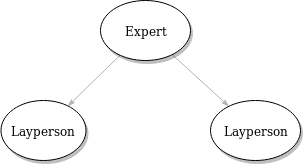
\includegraphics[width=0.5\textwidth]{Expert_Layperson.png}
	\caption{The minimalist setup of the present experiment.\label{fig:el}}
\end{figure}

\subsection{Setup}
The expert is much more likely to inquire correctly than the layperson is, this experiment uses values of $R_{\iota\varepsilon} = 0.85$ and $R_{\iota\a} = R_{\iota\beta} = 0.5$.

In each trial, both credences of the laypersons are set to the same uniformly distributed value. The experts initial credence is given by a beta-shaped meta distribution with a mean of $ 0.85$, meaning that on average over all trials the expert's initial credence is about that value.

The expert's trust in her own inquiry is set quite high, modeled here as a beta distribution with $\langle \tau^0_{\iota\varepsilon} \rangle = 0.85$ and a low $\sigma^2 = 0.005$, indicating that the expert isn't easily influenced in her trust in herself.

The laypersons are slightly overconfident, but more easily swayed, modeled as $\langle \tau^0_{\iota\a} \rangle =\langle \tau^0_{\iota\beta} \rangle = 0.55$ and $\sigma^2 = 0.01$.

The initial values $\langle \tau^0_{\varepsilon\a} \rangle =\langle \tau^0_{\varepsilon\beta} \rangle = 0.8$ with $\sigma^2 = 0.01$ are already quite high.

The assertion threshold, the threshold $T_A$ to recognize an authority and $\Delta_A$ have been set to $0.8, 0.82$ and $0.1$, respectively.

\subsection{Running the Experiment}

A single run of the experiment goes through the updating procedure for each agent as described above, through 10 discrete time steps. All changes in credence are recorded. For a snapshot of a single run of the program, see Fig.~\ref{fig:run} on page~\pageref{fig:run}.

\begin{figure}[ht]
	\centering
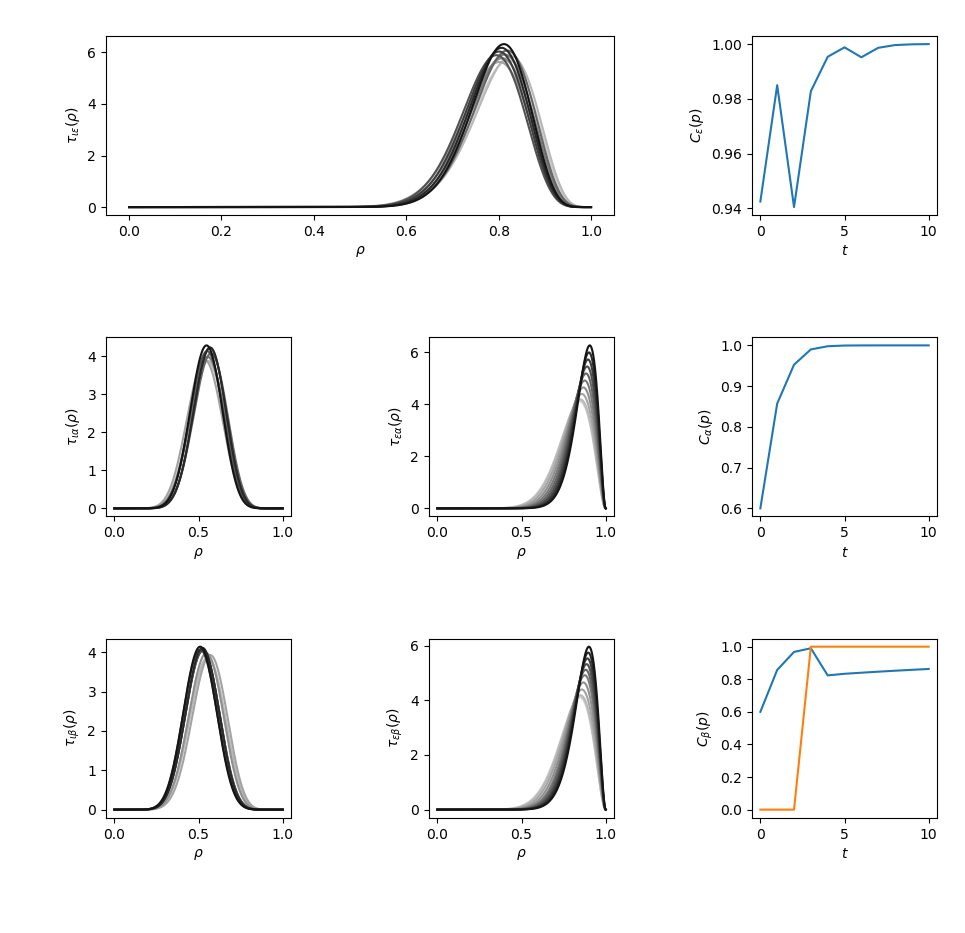
\includegraphics[width=\textwidth]{Run.png}
\caption{Example single run of the experiment with a layperson initial credence of $0.6$. The first row shows the expert's trust function in her own inquiry and her credence, the second row shows the Bayesianist's trust functions in herself and the expert as well as her credence. The third row shows the preemption strategist's trust functions and her credence. The orange line in the bottom right plot indicates whether she recognizes the expert as an authority (1 corresponds to yes). The increasing saturation of the black indicates time progress, the darker plots are later.\label{fig:run}}
\end{figure}

The experiment executes 10000 such runs, varying the starting conditions as described.

\section{Results}

\begin{figure}[h]
	\centering
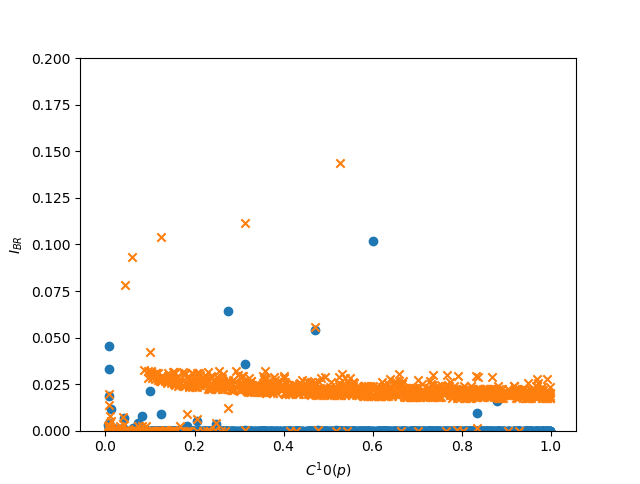
\includegraphics[width=0.8\textwidth]{Result.png}
\caption{Scatter plot of the result of (for legibility only) 1000 runs with the preemption strategist as orange X-markers. It seems that the starting credence has little effect on the Brier score after 10 steps, except for $C^{10} < 0.1$. In these cases, though, it is likely that the agent did not accept the expert as an authority.\label{fig:res}}
\end{figure}

To present the results it is necessary to compare the Brier Scores. Fig.~\ref{fig:res} gives a scatter plot of the results at $t=10$. After 10000 runs, the average Brier score of the preemption strategist was $\sim0.0254$, compared to the Bayesian's $\sim0.0076$, a stunning difference. An intuitive explanation for this result can be found by a look at Fig.~\ref{fig:run}, bottom right. Agent $\beta$ starts out Bayesian and quickly reaches a credence close to 1. Accordingly, her trust in the expert rises. As soon as the authority-threshold is reached, she drops her credence to $\langle \tau^0_{\varepsilon\a} \rangle $, then continuing to adapt her credence to the trust level. This procedure is a lot slower to approach 1 than the Bayesian, such that after 10 steps the Brier score is higher.

INTERPRETATION OF RESULTS (SHORT) AND WHAT CONCLUSIONS THIS RESULT LICENSES (NOT MANY)

\section{Caveats, Objections and Where to Go From Here}

- 
- the starting trust functions are kind of arbitrarily set and may influence the results. Should be put in parameter space and explored!

\nocite{*}
\printbibliography{}
\end{document}

